\documentclass[11pt]{article}

\usepackage{fullpage, graphicx, xcolor, wrapfig}

\graphicspath{{img}}


\begin{document}

\title{ARM Checkpoint... }
\author{Bartłomiej Cieślar, Jordan Hall, Ioana Mihăilescu and Oliver Killane}
\date{27/05/2021}

\maketitle

\section{Group Organisation}
    As the emulator and assembler are separate programs, that can be tested and implemented independently, we made a group decision to develop them in parallel.
    \begin{center}
        \begin{tabular}{ r | l }
            \textbf{Emulator} & \textbf{Assembler} \\
            Ioana \& Oliver & Bartłomiej \& Jordan \\
        \end{tabular}
    \end{center}
    \begin{center}
        \begin{tabular}{r l}
            Daily Standups & To bring up any issues with eachother's code, decide what to work on for the day. \\
            Status Diagram & Each function given a rating determining progress status. (\textcolor{red}{todo}/\textcolor{orange}{implemented}/\textcolor{green}{tested}) \\
            Merge Requests & New features done in separate branches, then merged into \textbf{emulate} to allow for reviews. \\
            Pair programming & Live on call, and with VSCode LiveShare to reduce bug incidence. \\
            Unit Tests & Create unit tests for separable functions as they are implemented. \\
        \end{tabular}
    \end{center}
    \subsection*{Development Cycle}
        \begin{center}
            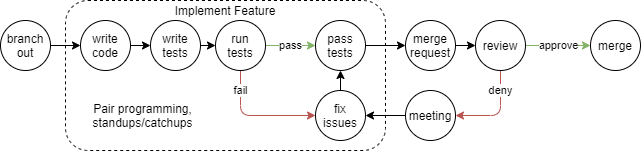
\includegraphics[width = \textwidth]{development cycle}
        \end{center}
    \subsection*{Group Function: \textcolor{green}{good}}
        By splitting the project and developing for predefined interfaces members can feel free to develop at their own pace, and for any given design decision at most two members can decide (too many cooks problem avoided).
        In particular pair programming has been very effective at writing bug-free, readable code on the first pass of our development cycle in most occasions.
        \newline\newline
        In the extension we will continue this strategy, but with the addition of more pair programming, in particular on test creation, as faulty unit tests have been a time consuming issue.
        \newline\newline
        One improvement we could make, is to delete and squash commits when merging a branch, this means we can preserve the commit message history, without having many 'dead' branches left following commits. Further using more descriptive branch names to ease confusion.

\section{Implementation Strategies}
    \subsection*{Project Structure}
        \begin{center}
            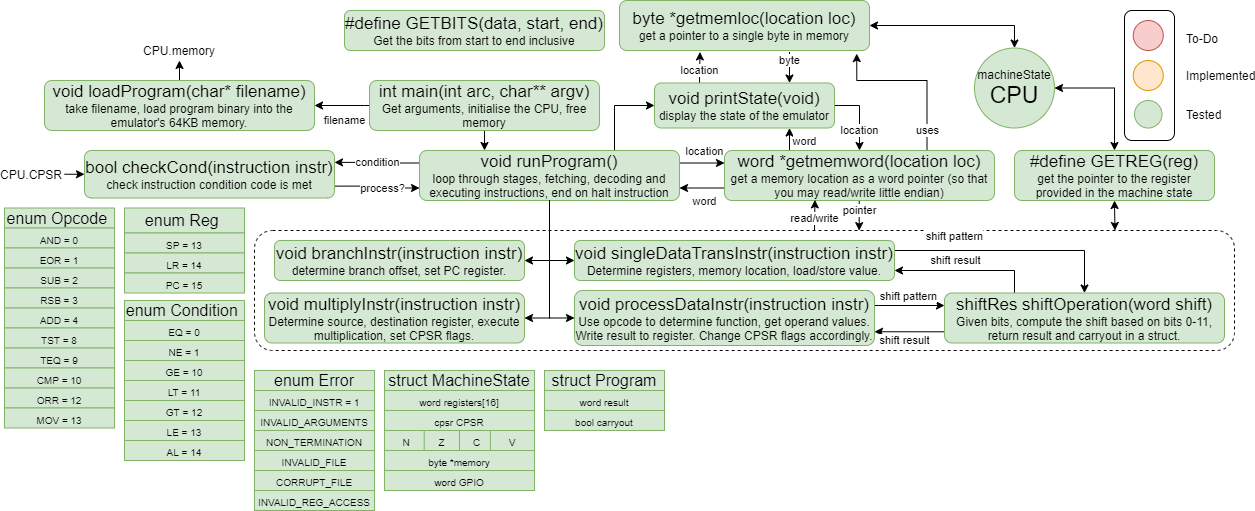
\includegraphics[width = \textwidth]{project status}
        \end{center}
    \begin{center}
        \begin{tabular}{l l l}
            Step & Functionality & Subroutine \\
            \hline
            (1) & Setup CPU, initialize values to zero. & \textcolor{green}{main} \\
            (2) & Read file into CPU memory. & \textcolor{green}{loadProgram}\\
            (3) & While not a halt instruction and no critical error: & \textcolor{green}{runProgram} \\
            (3a) & Read current instruction and increment PC.  & \textcolor{green}{runProgram}\\
            (3b) & Determine if instruction condition code is met by CPU CPSR register state. & \textcolor{green}{checkCond}\\
            (3c) & If so, determine instruction type.  & \textcolor{green}{runProgram}\\
            (3d) & Send instruction to appropriate function to change CPU state. & \textcolor{green}{Instr Functions}\\
            (4) & Display CPU state and exit. & \textcolor{green}{printState} \\
        \end{tabular}
    \end{center}
    The CPU state is held in a single global struct, for easy access. 


    



\end{document}
